% !TEX root = ../thesis.tex

\chapter{Conclusions and results}
\label{ch:results}

Thanks to the \texttt{\textbackslash subfloat} command, a single figure, such as \cref{fig:quadtree}, can contain multiple sub-figures with their own caption and referenceable separately as \cref{fig:mesh} and \cref{fig:polimi}. Use \texttt{TikZ} for high-quality hand-made figures, or just include external pictures as usual, with \verb|\includegraphics[options]{filename.png}|.

\vspace{\baselineskip}

\lipsum[1-5]

\begin{figure}
    \centering
    \subfloat[Quadtree mesh.\label{fig:mesh}]{
        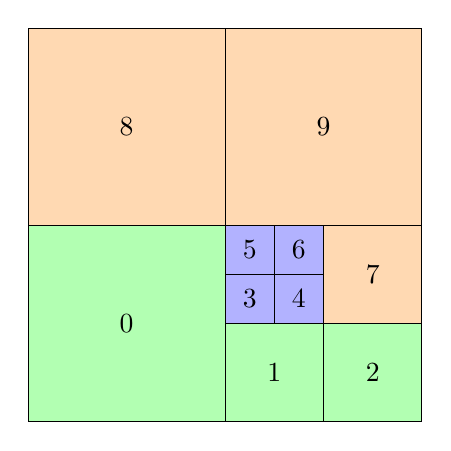
\begin{tikzpicture}[scale=1.25]
        \draw [fill={blue!30}] (2, 1) rectangle (2.5, 1.5);
        \draw [fill={blue!30}] (2.5, 1) rectangle (3, 1.5);
        \draw [fill={blue!30}] (2, 1.5) rectangle (2.5, 2);
        \draw [fill={blue!30}] (2.5, 1.5) rectangle (3, 2);
        \node [] at (2.25, 1.25) {3};
        \node [] at (2.75, 1.25) {4};
        \node [] at (2.25, 1.75) {5};
        \node [] at (2.75, 1.75) {6};
        
        \draw [fill={green!30}] (2, 0) rectangle (3, 1);
        \draw [fill={green!30}] (3, 0) rectangle (4, 1);
        \draw [fill={orange!30}] (3, 1) rectangle (4, 2);
        \node [] at (2.5, 0.5) {1};
        \node [] at (3.5, 0.5) {2};
        \node [] at (2.5, 1.5) {};
        \node [] at (3.5, 1.5) {7};
        
        \draw [fill={green!30}] (0, 0) rectangle (2, 2);
        \draw [fill={orange!30}] (0, 2) rectangle (2, 4);
        \draw [fill={orange!30}] (2, 2) rectangle (4, 4);
        \node [] at (1, 1) {0};
        \node [] at (3, 1) {};
        \node [] at (1, 3) {8};
        \node [] at (3, 3) {9};
        
        \draw (0, 0) rectangle node {} (4, 4);
        \end{tikzpicture}
    }
    \quad
    \subfloat[PoliMi logo.\label{fig:polimi}]{
        \includegraphics[scale=0.5]{polimi_logo.pdf}
    }
    \caption[Shorter caption]{This is a very long caption that you don't want to be displayed on the Table of Contents.}
    \label{fig:quadtree}
\end{figure}
